\documentclass{article}
\usepackage[pdftex]{graphicx,color}
\usepackage{amsmath}

% use the listings package for code snippets
\usepackage{listings}
\lstset{language=C++,basicstyle=\footnotesize}

% use the hyperref package; set the base for relative links to
% the top-level aspect directory so that we can link to
% files in the aspect tree without having to specify the
% location relative to the directory where the pdf actually
% resides
\usepackage[colorlinks,linkcolor=blue,urlcolor=blue,baseurl=../]{hyperref}

\newcommand{\dealii}{{\textsc{deal.II}}}
\newcommand{\pfrst}{{\normalfont\textsc{p4est}}}
\newcommand{\trilinos}{{\textsc{Trilinos}}}
\newcommand{\aspect}{\textsc{Aspect}}

\begin{document}

\thispagestyle{empty}
\vspace*{.3\textheight}

\begin{centering}
  \parindent0pt
  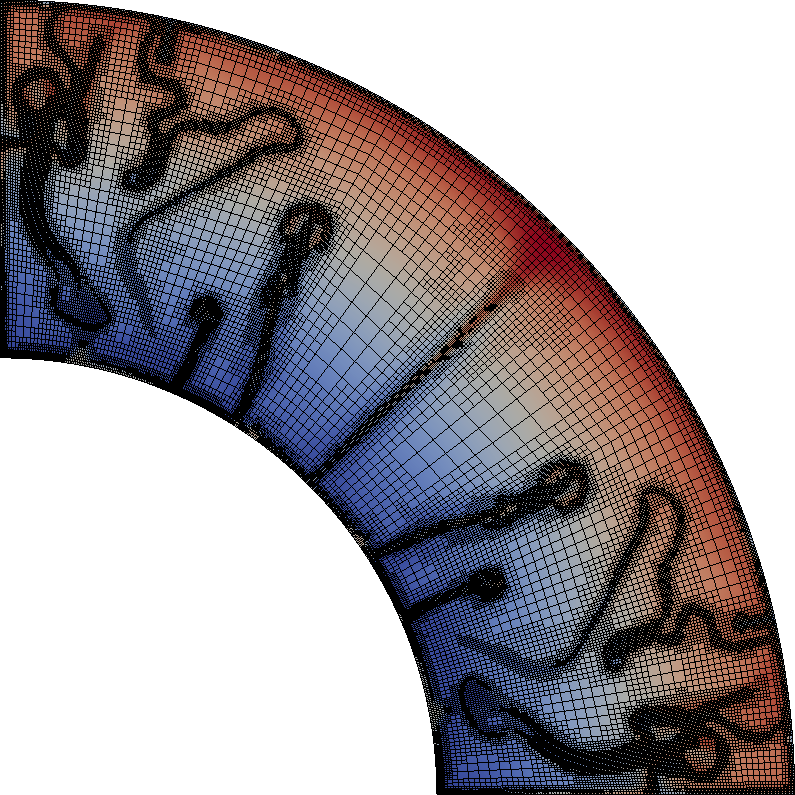
\includegraphics[width=0.6\textwidth]{mesh-2d.png}

  \vfill

  {\Large \aspect{} 0.8 preview release}
  \\[1cm]
  {\large
    Wolfgang Bangerth\\
    Timo Heister\\
    Martin Kronbichler\\
  }
\end{centering}


\pagebreak

\tableofcontents

\pagebreak

\section{Introduction}

\marginpar{To be written}

\section{Equations, models, coefficients}

\subsection{Basic equations}

\aspect{} solves the following system of equations in a two- or
three-dimensional domain $\Omega$:
\marginpar{To be finished}
\begin{align}
  \label{eq:stokes-1}
  -\nabla \cdot 2\eta \varepsilon(\mathbf u) + \nabla p &=
  \rho \mathbf g
  & \qquad
  & \textrm{in $\Omega$},
  \\
  \label{eq:stokes-2}
  \nabla \cdot (\rho \mathbf u) &= 0
  & \qquad
  & \textrm{in $\Omega$},
  \\
  \label{eq:temperature}
  \rho C_p \left(\frac{\partial T}{\partial t} + \mathbf u\cdot\nabla T\right)
  - \nabla\cdot k\nabla T
  &=
  \rho\gamma
  +
  2\eta \varepsilon(\mathbf u) : \varepsilon(\mathbf u)
  +
  C_p T \frac{D\rho}{Dt}?
  \ or \ \rho C_p \frac{\partial\rho}{\partial p} \mathbf u\cdot\mathbf g
  ...
  & \qquad
  & \textrm{in $\Omega$},
\end{align}
where $\varepsilon(\mathbf u) = \frac{1}{2}(\nabla \mathbf u + \nabla\mathbf
u^T)$ is the symmetric gradient of the velocity (often called the
\textit{strain rate}).

In this set of equations, \eqref{eq:stokes-1} and \eqref{eq:stokes-2}
represent the compressible Stokes equations in which $\mathbf u=\mathbf
u(\mathbf x,t)$ is the velocity field and $p=p(\mathbf x,t)$ the pressure
field. Both fields depend on space $\mathbf x$ and time $t$. Fluid flow is
driven by the gravity force that acts on the fluid and that is proportional to
both the density of the fluid and the strength of the gravitational pull.

Coupled to this Stokes system is equation \eqref{eq:temperature} for the
temperature field $T=T(\mathbf x,t)$ that contains heat conduction terms as
well as advection with the flow velocity $\mathbf u$.
.......talk about rhs

These equations are
augmented by boundary conditions that can either be of Dirichlet-, Neumann, or
tangential type on subsets of the boundary $\Gamma=\partial\Omega$:
\begin{align}
  \mathbf u &= 0 & \qquad &\textrm{on $\Gamma_{0,\mathbf u}$},
  \\
  \mathbf n \cdot \mathbf u &= 0 & \qquad &\textrm{on $\Gamma_{\parallel,\mathbf u}$},
  \\
  T &= T_{\text{prescribed}}
   & \qquad &\textrm{on $\Gamma_{D,T}$},
  \\
  \mathbf n \cdot k\nabla T &= 0
   & \qquad &\textrm{on $\Gamma_{N,T}$}.
\end{align}
Here,
$\Gamma_{0,\mathbf u}$ corresponds to parts of the boundary on which the
velocity is fixed to be zero,
$\Gamma_{\parallel,\mathbf u}$ to parts of the boundary on which the
velocity may be nonzero but must be parallel to the boundary,
where
$\Gamma_{D,T}$ to places where the temperature is prescribed (for example at
the inner and outer boundaries of the earth mantle), and finally
$\Gamma_{N,T}$ to places where the temperature is unknown but the heat flux
across the boundary is zero (for example on symmetry surfaces if only a part
of the shell that constitutes the domain the Earth mantle occupies is
simulated). We require that one of these boundary conditions hold at each
point for both velocity and temperature, i.e.,
$\Gamma_{0,\mathbf u}\cup\Gamma_{\parallel,\mathbf u}=\Gamma$ and
$\Gamma_{D,T}\cup\Gamma_{N,T}=\Gamma$.

\aspect{} solves these equations in essentially the form stated. In
particular, the form given in \eqref{eq:stokes-1} implies that the pressure
$p$ we compute is in fact the \textit{total pressure}, i.e., the sum of
hydrostatic pressure and dynamic pressure.%
\footnote{Other codes often replace this equation by $-\nabla \cdot 2\eta
  \nabla \mathbf u + \nabla p_d =
  (\rho-\rho_0) \mathbf g$ where $p_d=(p+\rho_0 \varphi)$, and $\phi$ is the
  gravitational potential so that
  $\mathbf g=-\nabla\varphi$ and chosen in such a way that $\varphi=0$ at that
  part of the boundary where we want the pressure to be zero (e.g., on the
  earth surface). Furthermore, $\rho_0$ is a reference density. In this
  formulation, it is clear that the quantity that drives the fluid flow is in
  fact the \textit{buoyancy} caused by the \textit{variation} of densities,
  not the density itself. $p_d=p+\rho_0 \varphi$ is then the \textit{dynamic}
  pressure, i.e., the difference between total pressure and hydrostatic
  pressure $p_s=-\rho_0\varphi$.

  While this formulation has a number of numerical advantages, it also has
  significant disadvantages: (i) The pressure we compute is not immediately
  comparable to quantities that we need to look up pressure-dependent
  quantities such as the density. (ii) The definition of a reference density
  is only simple if we have incompressible models for which the density only
  depends on the temperature; for more complicated models, it is not a priori
  clear which density $\rho_0$ to chose so that $p+\rho_0 \varphi$ really only
  contains the dynamic part of the pressure. (iii) To compute the total
  pressure $p$ from $p_d$ one needs to know a gravitational potential
  $\varphi$ that is consistent with the gravity vector $\mathbf g$. This is
  not always trivial because many simple models just prescribe a $\mathbf g$
  for which no such potential needs to exist; for example, this is the case
  when using a radially inward gravitational vector of constant magnitude.}
Consequently, it allows the direct use of this pressure when looking up
pressure dependent material parameters.

In the implementation of these equataions, \aspect{} uses the SI unit system
throughout (i.e., it expresses all quantities in meters, kilograms and seconds
-- the MKS system --, as well as degrees Kelvin). All material parameters,
geometries, etc., must also be expressed in these units. For convenience, some
rate-type output quantities are provided in units \textit{per year} instead of
\textit{per second}; however, this conversion happens at the time output is
generated, and is not part of the solution process.


\subsection{Coefficients}
\label{sec:coefficients}

The equations above contain a significant number of coefficients that we will
discuss in the following. In the most general form, many of these coefficients
depend nonlinearly on the solution variables pressure $p$, temperature $T$
and, in the case of the viscosity, on the strain rate $\varepsilon(\mathbf
u)$. Alternatively, they may be parameterized as a function of the spatial
variable $\mathbf x$. \aspect{} allows both kinds of parameterizations.

\textbf{Note: The next version of \aspect{} will actually iterate out
  nonlinearities in the material description. However, in the current version,
  we simply evaluate all nonlinear dependence of coefficients at the solution
  variables from the previous time step or a solution suitably extrapolated from
  the previous time steps.}

Note that below we will discuss examples of the dependence of coefficients on
other quantities; which dependence is actually implemented in the code is a
different matter. As we will discuss in Section~\ref{sec:parameters} and
\ref{sec:extending}, some versions of these models are already implemented and
can be selected from the input parameter file; others are easy to add to
\aspect{} by providing self-contained descriptions of a set of coefficients
that the rest of the code can then use without a need for further
modifications.

Concretely, we consider the following coefficients and dependencies:
\begin{itemize}
\item \textit{The viscosity $\eta=\eta(p,T,\varepsilon(\mathbf u),\mathbf
    x)$:} Units $\textrm{Pa}\cdot \textrm{s} =
  \textrm{kg}\frac{1}{\textrm{m}\cdot\textrm{s}}$.

  The viscosity is the proportionality factor that relates total forces
  (external gravity minus pressure gradients) and fluid velocities $\mathbf
  u$. The simplest models assume that $\eta$ is constant, with the constant
  often chosen to be on the order of $10^{21} \textrm{Pa}\;\textrm{s}$.

  More complex (and more realistic) models assume that the viscosity depends
  on pressure, temperature and strain rate. Since this dependence is often
  difficult to quantify, one modeling approach is to make $\eta$ spatially
  dependent.

\item \textit{The density $\rho=\rho(p,T,\mathbf x)$:} Units
  $\frac{\textrm{kg}}{\textrm{m}^3}$.

  In general, the density depends on pressure and temperature, both through
  pressure compression, thermal expansion, and phase changes the material may
  undergo as it moves through the pressure-temperature phase diagram.

  The simplest parameterization for the density is to assume a linear
  dependence on temperature, yielding the form
  $\rho(T)=\rho_{\text{ref}}[1-\beta (T-T_{\text{ref}})]$ where
  $\rho_{\text{ref}}$ is the reference density at temperature $T_{\text{ref}}$
  and $\beta$ is the linear thermal expansion coefficient. For the earth
  mantle, typical values for this parameterization would be
  $\rho_{\text{ref}}=3300\frac{\textrm{kg}}{\textrm{m}^3}$,
  $T_{\text{ref}}=293 \textrm{K}$, $\beta=2\cdot 10^{-5}
  \frac{1}{\mathrm{K}}$.

\item \textit{The gravity vector $\mathbf g=\mathbf g(\mathbf x)$:} Units
  $\frac{\textrm{m}}{\textrm{s}^2}$.

  Simple models assume a radially inward gravity vector of constant magnitude
  (e.g., the surface gravity of Earth, $9.81 \frac{\textrm{m}}{\textrm{s}^2}$),
  or one that can be computed analytically assuming a homogenous mantle
  density.

  A physically self-consistent model would compute the gravity vector as
  $\mathbf g = -\nabla \varphi$ with a gravity potential $\varphi$ that
  satisfies $-\Delta\varphi=4\pi G\rho$ with the density $\rho$ from above and
  $G$ the universal constant of gravity. This would provide a gravity vector
  that changes as a function of time. Such a model is not currently
  implemented.

\item \textit{The specific heat capacity $C_p=C_p(p,T,\mathbf x)$:} Units
  $\frac{\textrm{J}}{\textrm{kg}\cdot\textrm{K}} =
  \frac{\textrm{m}^2}{\textrm{s}^2\cdot\textrm{K}}$.

  The specific heat capacity denotes the amount of energy needed to increase
  the temperature of one kilogram of material by one degree. Wikipedia lists a
  value of 790 $\frac{\textrm{J}}{\textrm{kg}\cdot\textrm{K}}$ for granite%
  \footnote{See \url{http://en.wikipedia.org/wiki/Specific_heat}.}
  For the earth mantle, a value of 1250
  $\frac{\textrm{J}}{\textrm{kg}\cdot\textrm{K}}$ is within the range
  suggested by the literature.


\item \textit{The thermal conductivity $k=k(p,T,\mathbf x)$:} Units
  $\frac{\textrm{W}}{\textrm{m}\cdot\textrm{K}}=\frac{\textrm{kg}\cdot\textrm{m}}{\textrm{s}^3\cdot\textrm{K}}$.

  The thermal conductivity denotes the amount of thermal energy flowing
  through a unit area for a given temperature gradient. It depends on the
  material and as such will from a physical perspective depend on pressure and
  temperature due to phase changes of the material as well as through
  different mechanisms for heat transport (see, for example, the partial
  transparency of perovskite, the most abundant
  material in the earth mantle, at pressures above around 120 GPa
  \cite{BRVMFG04}).

  As a rule of thumb for its
  order of magnitude, wikipedia quotes values of
  $1.83$--$2.90\frac{\textrm{W}}{\textrm{m}\cdot\textrm{K}}$ for sandstone and
  $1.73$--$3.98\frac{\textrm{W}}{\textrm{m}\cdot\textrm{K}}$ for granite.%
  \footnote{See \url{http://en.wikipedia.org/wiki/Thermal_conductivity} and
    \url{http://en.wikipedia.org/wiki/List_of_thermal_conductivities}.} The
  values in the mantle are almost certainly higher than this though probably
  not by much. The exact exact value
  is not really all that important: heat transport through convection is
  several orders of magnitude more important than through thermal
  conduction.

\item \textit{The intrinsic specific heat production $\gamma=\gamma(\mathbf x)$:} Units
  $\frac{\textrm{W}}{\textrm{kg}}=\frac{\textrm{m}^2}{\textrm{s}^3}$.

  This term denotes the intrinsic heating of the material, for example due to
  the decay of radioactive material. As such, it depends not on pressure or
  temperature, but may depend on the location due to different chemical
  composition of material in the earth mantle. The literature suggests a value
  of $\gamma=7.4\cdot 10^{-12}\frac{\textrm{W}}{\textrm{kg}}$.
\end{itemize}


\subsection{Numerical methods}

There is no shortage in the literature for methods to solve the equations
outlined above. The methods used by \aspect{} use the following,
interconnected set of strategies in the implementation of numerical
algorithms:
\begin{itemize}
\item \textit{Mesh adaptation:} Mantle convection problems are characterized
  by widely disparate length scales (from plate boundaries on the order of
  kilometers or even smaller, to the scale of the entire earth). Uniform
  meshes can not resolve the smallest length scale without an intractable
  number of unknowns.  Fully adaptive meshes allow resolving local features of
  the flow field without the need to refine the mesh globally. Since the
  location of plumes that require high resolution change and move with time,
  meshes also need to be adapted every few time steps.
\item \textit{Accurate discretizations:} The Boussinesq problem upon which
  most models for the earth mantle are based
  has a number of intricacies that make the choice of discretization
  non-trivial. In particular, the finite elements chosen for velocity and
  pressure need to satisfy the usual compatibility condition for saddle point
  problems. This can be worked around using pressure stabilization schemes for
  low-order discretizations, but high-order methods can yield better accuracy
  with fewer unknowns and offer more reliability. Equally important is the choice of
  a stabilization method for the highly advection-dominated temperature
  equation. \aspect{} uses a nonlinear artificial diffusion method for the latter.
\item \textit{Efficient linear solvers:} The major obstacle in solving the
  Boussinesq system is the saddle-point nature of the Stokes equations. Simple
  linear solvers and preconditioners can not efficiently solve this system in
  the presence of strong heterogeneities or when the size of the system
  becomes very large. \aspect{} uses an efficient solution strategy based on a
  block triangular preconditioner utilizing an algebraic multigrid that
  provides optimal complexity even up to problems with hundreds of millions of
  unknowns.
\item \textit{Parallelization of all of the steps above:} Global mantle convection
  problems frequently require extremely large numbers of unknowns for
  adequate resolution in three dimensional simulations. The only realistic way to solve such problems lies in
  parallelizing computations over hundreds or thousands of processors. This is
  made more complicated by the use of dynamically changing meshes, and it
  needs to take into account that we want to retain the optimal complexity of
  linear solvers and all other operations in the program.
\item \textit{Modularity of the code:} A code that implements all of these
  methods from \textit{scratch} will be unwieldy, unreadable and unusable as a community
  resource. To avoid this, we build our implementation on widely used and well
  tested libraries that can provide researchers interested in extending it
  with the support of a large user community. Specifically, we use the
  \dealii{} library \cite{BHK07,BK99m} for meshes, finite
  elements and everything discretization related; the \trilinos{} library
  \cite{trilinos,trilinos-web-page} for scalable and parallel linear algebra;
  and \pfrst{} \cite{p4est} for distributed, adaptive meshes. As a
  consequence, our code is freed of the mundane tasks of defining finite
  element shape functions or dealing with the data structures of linear algebra,
  can focus on the high-level description of what is supposed to happen, and
  remains relatively compact. The code will also
  automatically benefit from improvements to the underlying libraries with
  their much larger development communities. \aspect{} is extensively
  documented to enable other researchers to understand, test, use, and extend it.
\end{itemize}

Rather than detailing the various techniques upon which \aspect{} is built, we
refer to the paper by Kronbichler, Heister and Bangerth \cite{KHB12} that
gives a detailed description and rationale for the various building blocks.



\subsection{Simplifications of the basic equations}

There are two common variations to equations
\eqref{eq:stokes-1}--\eqref{eq:temperature} that are frequently used and that
make the system much simpler to solve and analyze: assuming that the fluid is
incompressible (the Boussinesq approximation) and a linear dependence of the
density on the temperature with constants that are otherwise independent of
the solution variables. These are
discussed in the following; \aspect{} has
run-time parameters that allow both of these simpler models to be used.

\subsubsection{The Boussinesq approximation: Incompressibility}

The original Boussinesq approximation assumes that the density can be
considered constant in all occurrences in the equations with the exception of
the buoyancy term on the right hand side of \eqref{eq:stokes-1}. The primary
result of this assumption is that the continuity equation \eqref{eq:stokes-2}
will now read
\begin{gather*}
  \nabla \cdot \mathbf u = 0.
\end{gather*}
This makes the equations \textit{much} simpler to solve: First, because the
divergence operation in this equation is the transpose of the gradient of the
pressure in the momentum equation \eqref{eq:stokes-1}, making the system of
these two equations symmetric. And secondly, because the two equations are now
linear in pressure and velocity (assuming that the viscosity $\eta$ and the
density $\rho$ are considered fixed).

From a physical perspective, the assumption that the density is constant in
the continuity equation but variable in the momentum equation is of course
inconsistent. However, it is justified if the variation is small since the
momentum equation can be rewritten to read
\begin{gather*}
  -\nabla \cdot 2\eta \varepsilon(\mathbf u) + \nabla p_d =
  (\rho-\rho_0) \mathbf g,
\end{gather*}
where $p_d$ is the \textit{dynamic} pressure and $\rho_0$ is the constant
reference density. This makes it clear that the true driver of motion is in
fact the \textit{deviation} of the density from its background value, however
small this value is: the resulting velocities are simply proportional to the
density variation, not to the absolute magnitude of the density.

As such, the Boussinesq approximation can be justified. On the other hand,
given the real pressures and temperatures at the bottom of the earth mantle,
it is arguable whether the density can be considered to be almost
constant. Most realistic models predict that the density of mantle rocks
increases from somewhere around 3300 at the surface to over 5000 kilogram per
cubic meters at the core mantle boundary, due to the increasing lithostatic
pressure. While this appears to be a large variability, if the density changes
slowly with depth, this is not in itself an indication that the Boussinesq
approximation will be wrong. To this end, consider that the continuity
equation can be rewritten as $\frac 1\rho \nabla \cdot (\rho \mathbf u)=0$,
which we can multiply out to obtain
\begin{gather*}
  \nabla \cdot \mathbf u
  +
  \frac 1\rho \mathbf u \cdot \nabla \rho
  = 0.
\end{gather*}
The question whether the Boussinesq approximation is valid is then whether the
second term (the one omitted in the Boussinesq model) is small compared to the
first. To this end, consider that the velocity can change completely over length
scales of maybe 10 km, so that $\nabla \cdot\mathbf u \approx \|u\| /
10\text{km}$. On the other hand, given a smooth dependence of density on pressure,
the length scale for variation of the density is the entire earth mantle,
i.e., $\frac 1\rho\nabla \mathbf u \cdot \rho \approx \|u\| 0.5 / 3000 \text{km}$
(given a variation between minimal and maximal density of 0.5 times the
density itself). In other words, for a smooth variation, the contribution of
the compressibility to the continuity equation is very small. This may be
different, however, for models in which the density changes rather abruptly,
for example due to phase changes at mantle discontinuities.

As we will see in Section~\ref{sec:extending}, it is easy to add new material
models to \aspect. Each model can decide whether it wants to use the
Boussinesq approximation or not. The description of the models in
Section~\ref{parameters:Material_20model} also gives an answer which of the
models already implemented uses the approximation or considers the material
sufficiently compressible to go with the fully compressible continuity equation.


\subsubsection{Almost linear models}

\marginpar{To be written}

\section{Installation}

need deal.II, p4est, trilinos, mpi
unix-like system

see deal.II readme for instructions

currently need development version of deal.II


\section{Running \aspect}

Output in MKS, occasionally per year

\section{Input parameters}
\label{sec:parameters}

\subsection{Global parameters}
\label{parameters:global}


\begin{itemize}
\item {\it Parameter name:} {\tt CFL number}


{\it Value:} 1.0


{\it Default:} 1.0


{\it Description:} In computations, the time step $k$ is chosen according to $k = c \min_K \frac{h_K}{\|u\|_{\infty,K} p_T}$ where $h_K$ is the diameter of cell $K$, and the denominator is the maximal magnitude of the velocity on cell $K$ times the polynomial degree $p_T$ of the temperature discretization. The dimensionless constant $c$ is called the CFL number in this program. For time discretizations that have explicit components, $c$ must be less than a constant that depends on the details of the time discretization and that is no larger than one. On the other hand, for implicit discretizations such as the one chosen here, one can choose the time step as large as one wants (in particular, one can choose $c>1$) though a CFL number significantly larger than one will yield rather diffusive solutions. Units: None.


{\it Possible values:} [Double 0...1.79769e+308 (inclusive)]
\item {\it Parameter name:} {\tt End time}


{\it Value:} 2e8


{\it Default:} 1e8


{\it Description:} The end time of the simulation. Units: years.


{\it Possible values:} [Double 0...1.79769e+308 (inclusive)]
\item {\it Parameter name:} {\tt Output directory}


{\it Value:} output


{\it Default:} output


{\it Description:} The name of the directory into which all output files should be placed. This may be an absolute or a relative path.


{\it Possible values:} [DirectoryName]
\item {\it Parameter name:} {\tt Resume computation}


{\it Value:} false


{\it Default:} false


{\it Description:} A flag indicating whether the computation should be resumed from a previously saved state (if true) or start from scratch (if false).


{\it Possible values:} [Bool]
\end{itemize}



\subsection{Parameters in section \tt Boundary temperature model}
\label{parameters:Boundary_20temperature_20model}

\begin{itemize}
\item {\it Parameter name:} {\tt Model name}


{\it Value:} box


{\it Default:}


{\it Description:} Select one of the following models:

`spherical constant': A model in which the temperature is chosen constant on the
inner and outer boundaries of a spherical shell. Parameters are read from
subsection 'Spherical constant'.

`box': A model in which the temperature is chosen constant on the left and right sides of a box.


{\it Possible values:} [Selection spherical constant|box ]
\end{itemize}



\subsection{Parameters in section \tt Boundary temperature model/Spherical constant}
\label{parameters:Boundary_20temperature_20model/Spherical_20constant}

\begin{itemize}
\item {\it Parameter name:} {\tt Inner temperature}


{\it Value:} 6300


{\it Default:} 6000


{\it Description:} Temperature at the inner boundary (core mantle boundary). Units: K.


{\it Possible values:} [Double -1.79769e+308...1.79769e+308 (inclusive)]
\item {\it Parameter name:} {\tt Outer temperature}


{\it Value:} 300


{\it Default:} 0


{\it Description:} Temperature at the outer boundary (lithosphere water/air). Units: K.


{\it Possible values:} [Double -1.79769e+308...1.79769e+308 (inclusive)]
\end{itemize}

\subsection{Parameters in section \tt Discretization}
\label{parameters:Discretization}

\begin{itemize}
\item {\it Parameter name:} {\tt Stokes velocity polynomial degree}


{\it Value:} 2


{\it Default:} 2


{\it Description:} The polynomial degree to use for the velocity variables in the Stokes system. Units: None.


{\it Possible values:} [Integer range 1...2147483647 (inclusive)]
\item {\it Parameter name:} {\tt Temperature polynomial degree}


{\it Value:} 2


{\it Default:} 2


{\it Description:} The polynomial degree to use for the temperature variable. Units: None.


{\it Possible values:} [Integer range 1...2147483647 (inclusive)]
\item {\it Parameter name:} {\tt Use locally conservative discretization}


{\it Value:} false


{\it Default:} true


{\it Description:} Whether to use a Stokes discretization that is locally conservative at the expense of a larger number of degrees of freedom (true), or to go with a cheaper discretization that does not locally conserve mass, although it is globally conservative (false).


{\it Possible values:} [Bool]
\end{itemize}



\subsection{Parameters in section \tt Discretization/Stabilization parameters}
\label{parameters:Discretization/Stabilization_20parameters}

\begin{itemize}
\item {\it Parameter name:} {\tt alpha}


{\it Value:} 2


{\it Default:} 2


{\it Description:} The exponent $\alpha$ in the entropy viscosity stabilization. Units: None.


{\it Possible values:} [Double 1...2 (inclusive)]
\item {\it Parameter name:} {\tt beta}


{\it Value:} 0.078


{\it Default:} 0.078


{\it Description:} The $\beta$ factor in the artificial viscosity stabilization. An appropriate value for 2d is 0.052 and 0.078 for 3d. Units: None.


{\it Possible values:} [Double 0...1.79769e+308 (inclusive)]
\item {\it Parameter name:} {\tt cR}


{\it Value:} 0.5


{\it Default:} 0.11


{\it Description:} The $c_R$ factor in the entropy viscosity stabilization. Units: None.


{\it Possible values:} [Double 0...1.79769e+308 (inclusive)]
\end{itemize}

\subsection{Parameters in section \tt Geometry model}
\label{parameters:Geometry_20model}

\begin{itemize}
\item {\it Parameter name:} {\tt Model name}


{\it Value:} box


{\it Default:}


{\it Description:} Select one of the following models:

`spherical shell': A geometry representing a spherical shell or a piece of it.
Inner and outer radii are read from the parameter file in subsection 'Spherical
shell'.

`box': A box geometry with fixed length 1 in each coordinate direction.


{\it Possible values:} [Selection spherical shell|box ]
\end{itemize}



\subsection{Parameters in section \tt Geometry model/Spherical shell}
\label{parameters:Geometry_20model/Spherical_20shell}

\begin{itemize}
\item {\it Parameter name:} {\tt Inner radius}


{\it Value:} 5698e3


{\it Default:} 3481000


{\it Description:} Inner radius of the spherical shell. Units: m.


{\it Possible values:} [Double 0...1.79769e+308 (inclusive)]
\item {\it Parameter name:} {\tt Opening angle}


{\it Value:} 180


{\it Default:} 360


{\it Description:} Opening angle in degrees of the section of the shell that we want to build. Units: degrees.


{\it Possible values:} [Double 0...360 (inclusive)]
\item {\it Parameter name:} {\tt Outer radius}


{\it Value:} 10415e3


{\it Default:} 6336000


{\it Description:} Outer radius of the spherical shell. Units: m.


{\it Possible values:} [Double 0...1.79769e+308 (inclusive)]
\end{itemize}

\subsection{Parameters in section \tt Gravity model}
\label{parameters:Gravity_20model}

\begin{itemize}
\item {\it Parameter name:} {\tt Model name}


{\it Value:} vertical


{\it Default:}


{\it Description:} Select one of the following models:

`vertical': A gravity model in which the gravity direction is vertically downward and at constant magnitude.

`radial constant': A gravity model in which the gravity direction is radially inward and at constant magnitude. The magnitude is read from the parameter file in subsection 'Radial constant'.

`radial earth-like': A gravity model in which the gravity direction is radially inward and with a magnitude that matches that of the earth at the core-mantle boundary as well as at the surface and in between is physically correct under the assumption of a constant density.


{\it Possible values:} [Selection vertical|radial constant|radial earth-like ]
\end{itemize}



\subsection{Parameters in section \tt Gravity model/Radial constant}
\label{parameters:Gravity_20model/Radial_20constant}

\begin{itemize}
\item {\it Parameter name:} {\tt Magnitude}


{\it Value:} 30


{\it Default:} 30


{\it Description:} Magnitude of the gravity vector in $m/s^2$. The direction is always radially outward from the center of the earth.


{\it Possible values:} [Double 0...1.79769e+308 (inclusive)]
\end{itemize}

\subsection{Parameters in section \tt Initial conditions}
\label{parameters:Initial_20conditions}

\begin{itemize}
\item {\it Parameter name:} {\tt Model name}


{\it Value:} perturbed box


{\it Default:}


{\it Description:} Select one of the following models:

`spherical hexagonal perturbation': An initial temperature field in which the temperature is perturbed following a six-fold pattern in angular direction from an otherwise spherically symmetric state.

`spherical gaussian perturbation': An initial temperature field in which the temperature is perturbed by a single Gaussian added to an otherwise spherically symmetric state. Additional parameters are read from the parameter file in subsection 'Spherical gaussian perturbation'.

`perturbed box': An initial temperature field in which the temperature is perturbed slightly from an otherwise constant value equal to one. The perturbation is chosen in such a way that the initial temperature is constant to one along the entire boundary.


{\it Possible values:} [Selection spherical hexagonal perturbation|spherical gaussian perturbation|perturbed box ]
\end{itemize}



\subsection{Parameters in section \tt Initial conditions/Spherical gaussian perturbation}
\label{parameters:Initial_20conditions/Spherical_20gaussian_20perturbation}

\begin{itemize}
\item {\it Parameter name:} {\tt Amplitude}


{\it Value:} 0.01


{\it Default:} 0.01


{\it Description:} The amplitude of the perturbation.


{\it Possible values:} [Double 0...1.79769e+308 (inclusive)]
\item {\it Parameter name:} {\tt Angle}


{\it Value:} 4.71238898038468985769


{\it Default:} 0e0


{\it Description:} The angle where the center of the perturbation is placed.


{\it Possible values:} [Double 0...1.79769e+308 (inclusive)]
\item {\it Parameter name:} {\tt Non-dimensional depth}


{\it Value:} 0.7


{\it Default:} 0.7


{\it Description:} The non-dimensional radial distance where the center of the perturbation is placed.


{\it Possible values:} [Double 0...1.79769e+308 (inclusive)]
\item {\it Parameter name:} {\tt Sigma}


{\it Value:} 0.2


{\it Default:} 0.2


{\it Description:} The standard deviation of the Gaussian perturbation.


{\it Possible values:} [Double 0...1.79769e+308 (inclusive)]
\item {\it Parameter name:} {\tt Sign}


{\it Value:} 1


{\it Default:} 1


{\it Description:} The sign of the perturbation.


{\it Possible values:} [Double -1.79769e+308...1.79769e+308 (inclusive)]
\end{itemize}

\subsection{Parameters in section \tt Material model}
\label{parameters:Material_20model}

\begin{itemize}
\item {\it Parameter name:} {\tt Model name}


{\it Value:} simple


{\it Default:}


{\it Description:} Select one of the following models:

`table': A material model that reads tables of pressure and temperature dependent material coefficients from files.

`simple': A simple material model that has constant values for all coefficients but the density. This model uses the formulation that assumes an incompressible medium despite the fact that the density follows the law $\rho(T)=\rho_0(1-\beta(T-T_{\text{ref}})$. The value for the components of this formula and additional parameters are read from the parameter file in subsection 'Simple model'.


{\it Possible values:} [Selection table|simple ]
\end{itemize}



\subsection{Parameters in section \tt Material model/Simple model}
\label{parameters:Material_20model/Simple_20model}

\begin{itemize}
\item {\it Parameter name:} {\tt Reference density}


{\it Value:} 1


{\it Default:} 3300


{\it Description:} Reference density $\rho_0$. Units: $kg/m^3$.


{\it Possible values:} [Double 0...1.79769e+308 (inclusive)]
\item {\it Parameter name:} {\tt Reference temperature}


{\it Value:} 1


{\it Default:} 293


{\it Description:} The reference temperature $T_0$. Units: $K$.


{\it Possible values:} [Double 0...1.79769e+308 (inclusive)]
\item {\it Parameter name:} {\tt Thermal conductivity}


{\it Value:} 4.7


{\it Default:} 4.7


{\it Description:} The value of the thermal conductivity $k$. Units: $W/m/K$.


{\it Possible values:} [Double 0...1.79769e+308 (inclusive)]
\item {\it Parameter name:} {\tt Thermal expansion coefficient}


{\it Value:} 2e-5


{\it Default:} 2e-5


{\it Description:} The value of the thermal expansion coefficient $\beta$. Units: $1/K$.


{\it Possible values:} [Double 0...1.79769e+308 (inclusive)]
\item {\it Parameter name:} {\tt Viscosity}


{\it Value:} 1


{\it Default:} 5e24


{\it Description:} The value of the constant viscosity. Units: $kg/m/s$.


{\it Possible values:} [Double 0...1.79769e+308 (inclusive)]
\end{itemize}

\subsection{Parameters in section \tt Mesh refinement}
\label{parameters:Mesh_20refinement}

\begin{itemize}
\item {\it Parameter name:} {\tt Additional refinement times}


{\it Value:}


{\it Default:}


{\it Description:} A list of times so that if the end time of a time step is beyond this time, an additional round of mesh refinement is triggered. This is mostly useful to make sure we can get through the initial transient phase of a simulation on a relatively coarse mesh, and then refine again when we are in a time range that we are interested in and where we would like to use a finer mesh. Units: each element of the list has units years.


{\it Possible values:} [List list of <[Double 0...1.79769e+308 (inclusive)]> of length 0...4294967295 (inclusive)]
\item {\it Parameter name:} {\tt Coarsening fraction}


{\it Value:} 0.05


{\it Default:} 0.05


{\it Description:} The fraction of cells with the smallest error that should be flagged for coarsening.


{\it Possible values:} [Double 0...1 (inclusive)]
\item {\it Parameter name:} {\tt Initial adaptive refinement}


{\it Value:} 1


{\it Default:} 2


{\it Description:} The number of adaptive refinement steps performed after initial global refinement but while still within the first time step.


{\it Possible values:} [Integer range 0...2147483647 (inclusive)]
\item {\it Parameter name:} {\tt Initial global refinement}


{\it Value:} 4


{\it Default:} 2


{\it Description:} The number of global refinement steps performed on the initial coarse mesh, before the problem is first solved there.


{\it Possible values:} [Integer range 0...2147483647 (inclusive)]
\item {\it Parameter name:} {\tt Refinement fraction}


{\it Value:} 0.3


{\it Default:} 0.3


{\it Description:} The fraction of cells with the largest error that should be flagged for refinement.


{\it Possible values:} [Double 0...1 (inclusive)]
\item {\it Parameter name:} {\tt Time steps between mesh refinement}


{\it Value:} 5


{\it Default:} 10


{\it Description:} The number of time steps after which the mesh is to be adapted again based on computed error indicators.


{\it Possible values:} [Integer range 1...2147483647 (inclusive)]
\end{itemize}

\subsection{Parameters in section \tt Model settings}
\label{parameters:Model_20settings}

\begin{itemize}
\item {\it Parameter name:} {\tt Include shear heating}


{\it Value:} false


{\it Default:} true


{\it Description:} Whether to include shear heating into the model or not. From a physical viewpoint, shear heating should always be used but may be undesirable when comparing results with known benchmarks that do not include this term in the temperature equation.


{\it Possible values:} [Bool]
\item {\it Parameter name:} {\tt Radiogenic heating rate}


{\it Value:} 1


{\it Default:} 0e0


{\it Description:} H0


{\it Possible values:} [Double -1.79769e+308...1.79769e+308 (inclusive)]
\end{itemize}

\subsection{Parameters in section \tt Postprocess}
\label{parameters:Postprocess}

\begin{itemize}
\item {\it Parameter name:} {\tt List of postprocessors}


{\it Value:} all


{\it Default:} all


{\it Description:} A comma separated list of postprocessor objects that should be run at the end of each time step. Some of these postprocessors will declare their own parameters which may, for example, include that they will actually do something only every so many time steps or years. Alternatively, the text 'all' indicates that all available postprocessors should be run after each time step.

The following postprocessors are available:

`visualization': A postprocessor that takes the solution and writes it into files that can be read by a graphical visualization program. Additional run time parameters are read from the parameter subsection 'Visualization'.

`velocity statistics': A postprocessor that computes some statistics about the velocity field.

`temperature statistics': A postprocessor that computes some statistics about the temperature field.

`heat flux statistics': A postprocessor that computes some statistics about the heat flux across boundaries.


{\it Possible values:} [MultipleSelection visualization|velocity statistics|temperature statistics|heat flux statistics|all ]
\end{itemize}



\subsection{Parameters in section \tt Postprocess/Visualization}
\label{parameters:Postprocess/Visualization}

\begin{itemize}
\item {\it Parameter name:} {\tt Time between graphical output}


{\it Value:} 1


{\it Default:} 50


{\it Description:} The time interval between each generation of graphical output files. Units: years.


{\it Possible values:} [Double 0...1.79769e+308 (inclusive)]
\end{itemize}



\section{Extending \aspect}
\label{sec:extending}

\aspect{} is designed to be an extensible code. In particular, the program
uses a plugin architecture in which it is trivial to replace
or extend certain components of the program:
\begin{itemize}
\item the material description,
\item the geometry,
\item the gravity description,
\item the initial conditions,
\item the boundary conditions,
\item the functions that postprocess the solution.
\end{itemize}
We will discuss the way this is achieved in Section
\ref{sec:plugins}. Changing the core functionality, i.e., the basic equations
\eqref{eq:stokes-1}--\eqref{eq:temperature}, and how they are solved is
arguably more involved. We will discuss this in Section
\ref{sec:extending-solver}.

In either of these two cases, you will need to extend the source code of the
program. Since \aspect{} is written using the \dealii{} library, you will have
to familiarize yourself with this library for which there is an extensive
amount of documentation:
\begin{itemize}
\item The manual at
  \url{http://www.dealii.org/developer/doxygen/deal.II/index.html} that
  describes in detail what every class, function and variable in \dealii{}
  does.
\item A collection of modules at
  \url{http://www.dealii.org/developer/doxygen/deal.II/modules.html} that give
  an overview of whole groups of classes and functions and how they work
  together to achieve their goal.
\item The \dealii{} tutorial at
  \url{http://www.dealii.org/developer/doxygen/tutorial/index.html} that
  provides a step-by-step introduction to the library using a sequence of
  several dozen programs that introduce gradually more complex topics. In
  particular, you will learn \dealii's way of \textit{dimension independent
  programming} that allows you to write the program once, test it in 2d, and
  run the exact same code in 3d without having to debug it a second time.
\item The step-31 and step-32 tutorial programs at
  \url{http://www.dealii.org/developer/doxygen/deal.II/step_31.html} and
  \url{http://www.dealii.org/developer/doxygen/deal.II/step_32.html} from
  which \aspect{} directly descends.
\item The \dealii{} Frequently Asked Questions at
  \url{http://dealii.sourceforge.net/index.php/Deal.II_Questions_and_Answers}
  that also have extensive sections on developing code with \dealii{} as well
  as on debugging.
\item Several other parts of the \dealii{} website at
  \url{http://www.dealii.org/} also have information that may be relevant if
  you dive deeper into developing code. If you have questions, the mailing
  lists at \url{http://www.dealii.org/mail.html} are also of general help.
\end{itemize}

As a general note, \aspect{} utilizes a \dealii{} feature called \textit{debug
  mode}. By default, \aspect{} uses debug mode, i.e., it calls a version of
the \dealii{} library that contain lots of checks for the correctness of
function arguments, the consistency of the internal state of data structure,
etc. If you program with \dealii{}, for example to extend \aspect{}, it has
been our experience over the years that, by number, most programming errors are of the
kind where one forgets to initialize a vector, one accesses data that has not
been updated, one tries to write into a vector that has ghost elements,
etc. If not caught, the result of these bugs is that parts of the program use
invalid data (data written into ghost elements is not communicated to other
processors), that operations simply make no sense (adding vectors of different
length), that memory is corrupted (writing past the end of an array) or, in
rare and fortunate cases, that the program simply crashes.

Debug mode is designed to catch most of these errors: It enables some 7,300
assertions (as of late 2011) in \dealii{} where we check for errors like the
above and, if the condition is violated, abort the program with a detailed
message that shows the failed check, the location in the source code, and a
stacktrace how the program got there. When you write new functionality and run
the code for the first time, you will almost invariably first have to deal
with a number of these assertions that point out problems in your code. While
this may be annoying at first, remember that these are actual bugs in your
code that have to be fixed anyway and that are much easier to find if the
program aborts than if you have to go by their more indirect results such as
wrong answers. The Frequently Asked Questions at
\url{http://dealii.sourceforge.net/index.php/Deal.II_Questions_and_Answers}
contain a section on how to debug \dealii{} programs.

The downside of debug mode is that it makes the program much slower --
depending on application by a factor of 4--10. Consequently, once you are
confident that your program actually does what it is intended to do --
\textbf{but no earlier!} --, you may want to switch to optimized mode that
links \aspect{} with a version of the \dealii{} libraries that uses compiler
optimizations and that does not contain the \texttt{assert} statements
discussed above. This switch can be facilitated by editing the top of the
\aspect{} \url{Makefile} and recompiling the program.

In addition to these general comments, \aspect{} is itself extensively
documented. You can find documentation on all classes, functions and
namespaces starting from the \url{doc/doxygen/index.html} page.


\subsection{Materials, geometries, gravitation and other aspects of the model:
  plugins}
\label{sec:plugins}

The most common modification you will probably want to do to \aspect{} are to
switch to a different material model (i.e., have different values of
functional dependencies for the coefficients $\eta,\rho,C_p, \ldots$ discussed
in Section~\ref{sec:coefficients}); change the geometry; change the direction
and magnitude of the gravity vector $\mathbf g$; or change the initial and
boundary conditions.

To make this as simple as possible, all of these parts of the program have
been separated into modules that can be replaced quickly and where it is
simple to add a new implementation and make it available to the rest of the
program and the input parameter file. The way this is achieved is through the
following two steps:
\begin{itemize}
\item The rest of the program only communicates with material models,
  geometry descriptions, etc., through a simple and very basic
  interface. These interfaces are declared in the files
  \url{include/aspect/material_model/interface.h},
  \url{include/aspect/geometry_model/interface.h}, etc., header files. These
  classes are always called \texttt{Interface}, are located in namespaces that
  identify their purpose, and their documentation can be found from the
  general class overview in \url{doc/doxygen/classes.html}.

  To show an example of a rather minimal case, here is the declaration of the
  \texttt{aspect::GravityModel::Interface} class (documentation comments have
  been removed):
  \begin{lstlisting}[frame=single]
    class Interface
    {
      public:
        virtual ~Interface();

        virtual
        Tensor<1,dim>
        gravity_vector (const Point<dim> &position) const = 0;

        static void declare_parameters (ParameterHandler &prm);

        virtual void parse_parameters (ParameterHandler &prm);
    };
  \end{lstlisting}

  If you want to implement a new model for gravity, you just need to write a
  class that derives from this base class and implements the
  \texttt{gravity\_vector} function. If your model wants to read parameters
  from the input file, you also need to have functions called
  \texttt{declare\_parameters} and \texttt{parse\_parameters} in your class
  with the same signatures as the ones above.

  Each of the categories above that allow plugins have several implementations
  of their respective interfaces that you can use to get an idea how to
  implement a new model.

\item At the end of the file where you implement your new model, you need to
  have a call to the macro \texttt{ASPECT\_REGISTER\_GRAVITY\_MODEL}. For
  example, let us say that you had implemented a gravity model that takes
  actual gravimetric readings from the GRACE satellites into account, and had
  put everything that is necessary into a class
  \texttt{aspect::GravityModel::GRACE}. Then you need a statement like this at
  the bottom of the file:
  \begin{lstlisting}[frame=single]
    ASPECT_REGISTER_GRAVITY_MODEL
    (GRACE,
     "grace",
     "A gravity model derived from GRACE "
     "data. Run-time parameters are read from the parameter "
     "file in subsection 'Radial constant'.");
  \end{lstlisting}
  Here, the first argument to the macro is the name of the class. The second
  is the name by which this model can be selected in the parameter file. And
  the third one is a documentation string that describes the purpose of the
  class (see, for example, Section~\ref{parameters:Gravity_20model} for an
  example of how existing models describe themselves).

  This little piece of code ensures several things: (i) That the parameters
  this class declares are known when reading the parameter file. (ii) That you
  can select this model (by the name ``grace'') via the run-time parameter
  \texttt{Gravity model/Model name}. (iii) That \aspect{} can create an object
  of this kind when selected in the parameter file.

  Note that you need not announce the existence of this class in any other
  part of the code: Everything should just work automatically. Note also that
  the existing implementations of models of the gravity and other interfaces
  declare the class in a header file and define the member functions in a
  \texttt{.cc} file. This is done so that these classes show up in our
  doxygen-generated documentation, but it is not necessary: you can put your
  entire class declaration and implementation into a single file as long as
  you call the macro discussed above on it.
\end{itemize}

The procedure for the other areas where plugins are supported works
essentially the same, with the obvious change in namespace for the interface
class and macro name.

In the following, we will discuss the requirements for individual plugins.


\subsubsection{Material models}
\subsubsection{Geometry models}
\subsubsection{Gravity models}
\subsubsection{Initial conditions}
\subsubsection{Boundary conditions}
\subsubsection{Postprocessors: Evaluating the solution after each time step}

\subsection{Extending the basic solver}
\label{sec:extending-solver}

step-31/32

\bibliographystyle{alpha}
\bibliography{manual}

\end{document}
